\documentclass[12pt,t]{beamer}
\usetheme[greyauthor, % Grå tekst forfatter som KU vil have
         unit=NAT, % Ændre til NAT, KU, eller unit=ics (diku)
         dk, % Sprog
         %style=simple, % Vandmærke eller billede
         footstyle=low, % Fjern stor footer
         wmark, % vandmærke på hver side
         logoplace=left % Logo til venstre
         %,sidebar % makes sidebar
         ]{Frederiksberg}
% nat for Science, ku for generic or unit=ics for DIKU
% Tilføj style=simple for vandmærke
\usepackage{listings} % Pakke til kode
\usepackage{pslatex}        % pæn skrift
\usepackage[utf8]{inputenc} % Implementerer Unicode
\usepackage{algpseudocode}
\usepackage{algorithm}

\title{ATU besøg på DIKU}
\subtitle{Algoritmer og problemløsning}
\author{
        Arinbjörn Brandsson \\
        Benjamin Rotendahl  \\
        Mathias Fleig Mortensen \\
        Christopher Mulvad Groot
}

\date[]{\today}


\begin{document}

\frame[plain]{\titlepage}

\begin{frame}[t]{Eksempler på køretid}
    \vspace{-2em}
    \begin{columns}
        \begin{column}{0.33\textwidth}
            \begin{block}{Bogo Sort}
                \begin{itemize}
                    \item Køretid på $O(n!)$
                \end{itemize}
            \end{block}
        \end{column}
        \begin{column}{0.33\textwidth}
            \begin{block}{Insertion Sort}
                \begin{itemize}
                    \item Køretid? $O(n^2)$
                \end{itemize}
            \end{block}
        \end{column}

        \begin{column}{0.33\textwidth}
            \begin{block}{Merge sort}
                \begin{itemize}
                    \item Køretid på $O(n \lg n)$
                \end{itemize}
            \end{block}
        \end{column}
    \end{columns}
    \begin{figure}[h!]
        \caption{Graf over køretider}
        \centering
        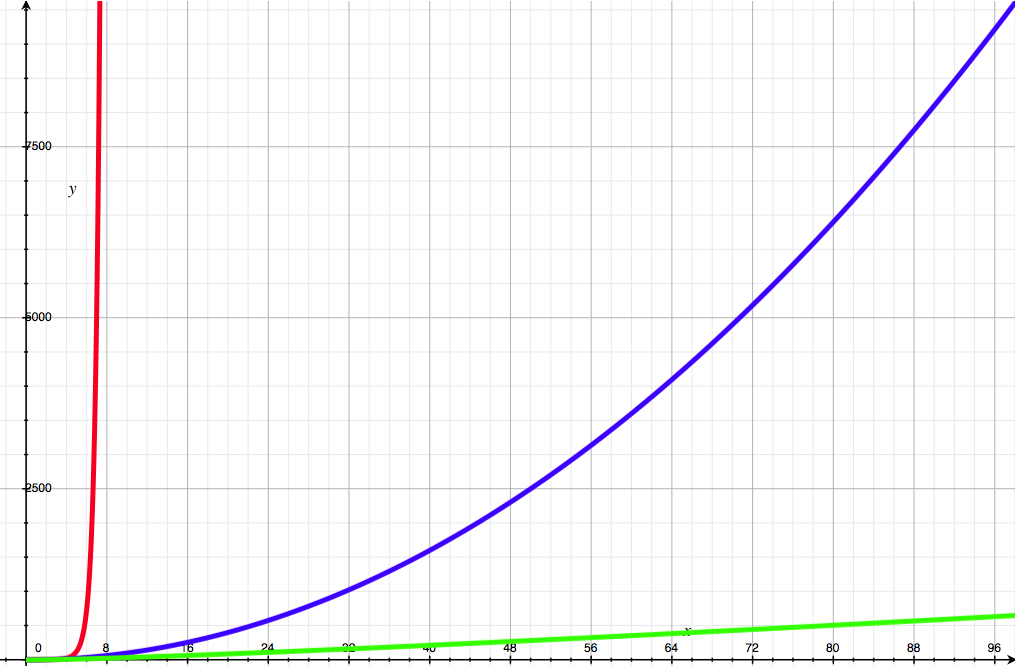
\includegraphics[width=0.7\textwidth]{./include/exs.png}
    \end{figure}
\end{frame}

\section{Fibonacci Tal}
    \begin{frame}[c]{Overlappende under problemer}
        \begin{block}{Eksempel}
            Det $n$'te\emph{Fibonacci} tal er defineret som summen af de to
            forgående.
            $$
              1,1,2,3,5,8,13,21,34,55, \dots
            $$
            \pause
            Hvordan bestemmer vi dem?
        \end{block}
    \end{frame}

    \begin{frame}[c]{Sommer i Sunny beach}
        \begin{block}{Beskrivelse}
          Det er sommer i \emph{Sunny Beach} og en kæde af barer langs kysten
          har et problem,\pause  de kan ikke bestille flere øl!
          \\
          \pause  ~ \\
          Hver bar langs strandvejen har $b_i$ øl tilbage, der er ikke
          nogen der ved hvilken bar der kan sælge flest øl på en given aften.
          \pause
          Det er besluttet at alle barer skal have lige mange øl. \\
          \pause
          ~\\
          De har en lastbil hvor der kan være en uendelig mængde af øl, \pause
          dog er vognførererne på denne lastbil glade for øl. Hver gang der er
          kørt en kilometer så drikkes der to øl.
        \end{block}
    \end{frame}

    \begin{frame}[c]{Eksempel}
        \begin{block}{Figur}
          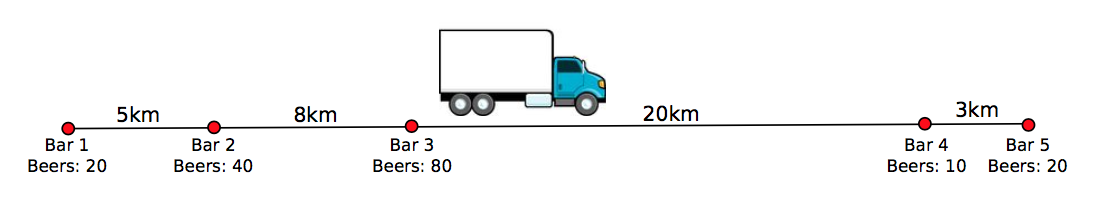
\includegraphics[scale=0.5]{fragt.png}
        \end{block}
        \pause
        \begin{block}{Hvad i får som input}
          \begin{itemize}
            \item En liste over hvor mange øl der er på hver bar $b_1, b_2, \dots$
            \item En liste over afstanden mellem dem $a_1, a_2, \dots$ \pause
            \item Det antal øl de gerne vil have på hver bar \pause
          \end{itemize}
        \end{block}

        \begin{block}{Hvad i skal svare}
          \begin{itemize}
            \item ja, eller nej. \pause
            \item Svar også på hvordan man kan finde det optimale antal.
          \end{itemize}
        \end{block}
    \end{frame}

    \begin{frame}{DNS system}
    \begin{block}{Hvad er DNS}
        Forklaring på tavlen
    \end{block}
      \begin{block}{Mål}
          Tænk over hvordan vi kan lave et DNS system
      \end{block}
      \pause
      \begin{exampleblock}{Eksempel}
          Snak lidt om hvordan det kunne gøre smart
      \end{exampleblock}
    \end{frame}

    \begin{frame}[plain]{Zig-Zag sekvens}
        \begin{block}{Beskrivelse}
          Ejeren af et supermarked har fået en ny stor ølhylde, nu vil han gerne
          gøre den pæn. Han har placeret sine øl i alfabetisk orden, men højden
          på flaskerne afviger. Han er nu intereseret i at finde den længste
          sekvens af øl der skifter mellem lav og høj en såkaldt Zig-Zag sekvens.
          Så $(15,10,17)$ er sådan en sekvens mens $(1,2,3)$ ikke er.

          Vi skal lave en algoritme der bestemmer sådan en sekvens.\\
          \textbf{Input:} $n$ øl flaskers højde $n_1, n_2, \dots$. \\
          \textbf{Output:} Den længst mulige Zig-Zag sekvens.
        \end{block}
    \end{frame}

    \begin{frame}
      \begin{columns}
          \begin{column}{0.5\textwidth}
              \begin{block}{Eksempel}
                \begin{itemize}
                    \item Input : $(6, 1, 7, 7, 2, 4, 7)$
                    \item Output : $(6,1,7,2,7)$
                \end{itemize}
              \end{block}
          \end{column}
          \begin{column}{0.5\textwidth}
              \begin{block}{Figur}
                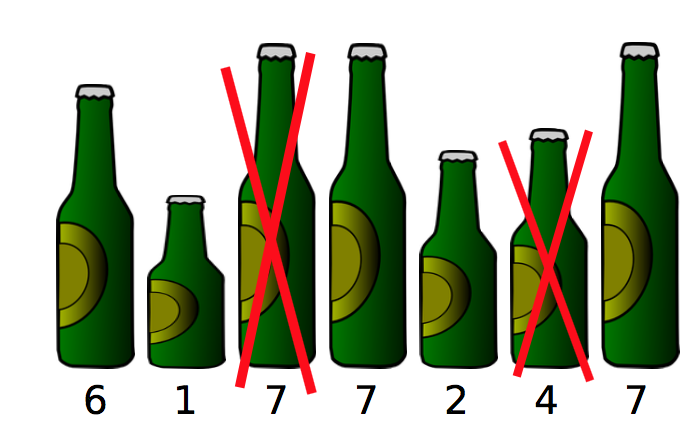
\includegraphics[scale=0.3]{oel.png}
              \end{block}
          \end{column}
      \end{columns}
        I må gerne fjerne flasker men ikke bytte rundt på dem, beskriv en metode
        til at bestemme den her sekvens og tænk over hvor effektivt den er.
    \end{frame}


    \begin{frame}{Primtal}
      \begin{block}{Mål}
      Skriv en algoritme der finder det $n$'te primtal --- prøv at gør den så
      hurtig som mulig.
      \end{block}
      \pause

      \begin{exampleblock}{Eksempel}
      Find det femte primtal. Algoritmen skal gerne returnere 11.
      \end{exampleblock}
    \end{frame}


\end{document}
